% =============================================================================
%  Diplomado en Data Science Aplicada con Python para la Toma de Decisiones
%  Clase 9: Estadística Descriptiva — Distribuciones, Dispersión y Outliers
%  Arca Continental Ecuador | UDLA
%
%  Compilar: pdflatex -shell-escape presentacion.tex (x2 para refs)
% =============================================================================
\documentclass[aspectratio=169, 11pt]{beamer}

\usepackage[T1]{fontenc}
\usepackage[utf8]{inputenc}
\usepackage[spanish,es-noshorthands]{babel}
\usepackage{FiraSans}
\usepackage{FiraMono}
\renewcommand{\familydefault}{\sfdefault}
\usepackage{graphicx}
\usepackage{tikz}
\usetikzlibrary{arrows.meta, positioning, shapes.geometric, shapes.misc,
  calc, fit, decorations.pathreplacing, backgrounds}
\usepackage{fontawesome5}
\usepackage{minted}
\usepackage{tcolorbox}
\tcbuselibrary{minted, skins, breakable}
\usepackage{booktabs}
\usepackage{colortbl}
\usepackage{multicol}
\usepackage{hyperref}
\usepackage{calc}
\usepackage{amsmath}

\definecolor{arcaRed}{HTML}{C82B40}
\definecolor{arcaDark}{HTML}{6B1525}
\definecolor{udlaCrimson}{HTML}{A31545}
\definecolor{arcaGray}{HTML}{F5F5F5}
\definecolor{arcaLightGray}{HTML}{EBEBEB}
\definecolor{textDark}{HTML}{2D2D2D}
\definecolor{textMuted}{HTML}{6B7280}
\definecolor{codeGreen}{HTML}{16A34A}
\definecolor{codeBlue}{HTML}{2563EB}
\definecolor{codeOrange}{HTML}{EA580C}
\definecolor{codePurple}{HTML}{7C3AED}

\usetheme{default}
\usecolortheme{default}
\setbeamertemplate{navigation symbols}{}
\setbeamertemplate{footline}{}
\setbeamertemplate{headline}{}
\setbeamercolor{normal text}{fg=textDark}
\setbeamercolor{frametitle}{fg=arcaRed, bg=white}
\setbeamercolor{title}{fg=white}
\setbeamercolor{subtitle}{fg=white!85}
\setbeamercolor{author}{fg=white!80}
\setbeamercolor{date}{fg=white!70}
\setbeamercolor{item}{fg=arcaRed}
\setbeamercolor{subitem}{fg=arcaDark}
\setbeamercolor{block title}{fg=white, bg=arcaRed}
\setbeamercolor{block body}{fg=textDark, bg=arcaGray}
\setbeamercolor{block title alerted}{fg=white, bg=codeOrange}
\setbeamercolor{block body alerted}{fg=textDark, bg=arcaGray}
\setbeamercolor{block title example}{fg=white, bg=codeGreen}
\setbeamercolor{block body example}{fg=textDark, bg=arcaGray}
\setbeamercolor{section in toc}{fg=arcaDark}
\setbeamerfont{frametitle}{size=\Large, series=\bfseries}
\setbeamerfont{title}{size=\huge, series=\bfseries}
\setbeamerfont{subtitle}{size=\large}
\setbeamerfont{author}{size=\normalsize}
\setbeamerfont{date}{size=\small}
\setbeamerfont{block title}{size=\normalsize, series=\bfseries}
\setbeamerfont{footnote}{size=\tiny}
\setbeamertemplate{itemize item}{\scriptsize\raise1.5pt\hbox{\color{arcaRed}$\blacktriangleright$}}
\setbeamertemplate{itemize subitem}{\scriptsize\raise1pt\hbox{\color{arcaDark}$\bullet$}}
\setbeamertemplate{enumerate items}[default]
\setbeamercolor{enumerate item}{fg=arcaRed}

\setbeamertemplate{headline}{%
  \begin{tikzpicture}[remember picture, overlay]
    \fill[arcaDark] (current page.north west) rectangle
      ([yshift=-0.7cm]current page.north east);
    \node[anchor=west, inner sep=0pt] at
      ([xshift=0.6cm, yshift=-0.35cm]current page.north west)
      {
\includegraphics[height=0.45cm]{../logo_udla_white.png}};
    \node[anchor=east, inner sep=0pt] at
      ([xshift=-0.6cm, yshift=-0.35cm]current page.north east)
      {
\includegraphics[height=0.45cm]{../ArcaContinental_white.png}};
  \end{tikzpicture}%
  \vspace{0.7cm}%
}

\setbeamertemplate{footline}{%
  \begin{tikzpicture}[remember picture, overlay]
    \node[anchor=south east, font=\scriptsize\bfseries\color{arcaRed}] at
      ([xshift=-0.5cm, yshift=0.15cm]current page.south east)
      {\insertframenumber};
  \end{tikzpicture}%
  \vspace{0.3cm}%
}

\setbeamertemplate{frametitle}{%
  \vspace{0.25cm}%
  \usebeamerfont{frametitle}\usebeamercolor[fg]{frametitle}\insertframetitle%
  \par\vspace{2pt}%
  \begin{tikzpicture}
    \fill[arcaRed] (0,0) rectangle (3cm, 1.5pt);
    \fill[arcaLightGray] (3cm,0) rectangle (\textwidth, 0.5pt);
  \end{tikzpicture}%
  \vspace{0.1cm}%
}

\newtcblisting{pyblock}[1][]{%
  listing engine=minted, minted language=python, minted style=friendly,
  minted options={fontsize=\small, linenos=false, breaklines=true, python3=true},
  colback=arcaGray, colframe=arcaRed, left=4pt, right=4pt, top=4pt, bottom=4pt,
  boxrule=0pt, leftrule=3pt, arc=2pt, listing only, #1}

\newtcblisting{outputblock}[1][]{%
  listing engine=minted, minted language=text, minted style=bw,
  minted options={fontsize=\small, breaklines=true},
  colback=white, colframe=arcaLightGray, left=4pt, right=4pt, top=4pt, bottom=4pt,
  boxrule=0.5pt, arc=2pt, listing only,
  title={\small\faTerminal\hspace{6pt}Output}, coltitle=textMuted,
  fonttitle=\small\ttfamily, colbacktitle=white, #1}

\newcommand{\sectionframe}[2]{%
  \begingroup
  \setbeamertemplate{headline}{}%
  \setbeamertemplate{footline}{}%
  \begin{frame}[plain, noframenumbering]
    \begin{tikzpicture}[remember picture, overlay]
      \fill[arcaRed] (current page.south west) rectangle (current page.north east);
      \node[anchor=center, text=white, font=\Huge\bfseries, text width=12cm,
            align=center] at ([yshift=0.5cm]current page.center) {#1};
      \node[anchor=center, text=white!80, font=\large, text width=10cm,
            align=center] at ([yshift=-0.8cm]current page.center) {#2};
    \end{tikzpicture}
  \end{frame}
  \endgroup
}

\title{Diplomado en Data Science Aplicada\\con Python para la Toma de Decisiones}
\subtitle{Clase 9: Estadística Descriptiva --- Distribuciones, Dispersión y Outliers}
\author{Carlos Enrique Mosquera Trujillo}
\date{27 de Marzo, 2026}

\begin{document}

% ── PORTADA ──────────────────────────────────────────────────────────────────
{
\setbeamertemplate{headline}{}
\setbeamertemplate{footline}{}
\begin{frame}[plain, noframenumbering]
  \begin{tikzpicture}[remember picture, overlay]
    \fill[arcaDark] (current page.south west) rectangle (current page.north east);
    \fill[arcaRed] ([yshift=-3.5cm]current page.north west) rectangle
      ([yshift=-4.2cm]current page.north east);
    \node[anchor=west, inner sep=0pt] at
      ([xshift=1cm, yshift=-1.5cm]current page.north west)
      {
\includegraphics[height=1cm]{../logo_udla_white.png}};
    \node[anchor=east, inner sep=0pt] at
      ([xshift=-1cm, yshift=-1.5cm]current page.north east)
      {
\includegraphics[height=1cm]{../ArcaContinental_white.png}};
  \end{tikzpicture}
  \vspace{2.5cm}
  \begin{center}
    {\usebeamerfont{title}\usebeamercolor[fg]{title}\inserttitle\par}
    \vspace{0.4cm}
    {\usebeamerfont{subtitle}\usebeamercolor[fg]{subtitle}\insertsubtitle\par}
    \vspace{0.6cm}
    {\usebeamerfont{author}\usebeamercolor[fg]{author}\insertauthor\par}
    \vspace{0.15cm}
    {\usebeamerfont{date}\usebeamercolor[fg]{date}\insertdate\par}
  \end{center}
\end{frame}
}

% ── MÓDULO 2 ─────────────────────────────────────────────────────────────────
{
\setbeamertemplate{headline}{}
\setbeamertemplate{footline}{}
\begin{frame}[plain, noframenumbering]
  \begin{tikzpicture}[remember picture, overlay]
    \fill[arcaDark] (current page.south west) rectangle (current page.north east);
    \node[anchor=center, text=white, font=\Large\bfseries, text width=12cm,
          align=center] at ([yshift=1cm]current page.center)
      {Módulo 2};
    \node[anchor=center, text=white!90, font=\huge\bfseries, text width=12cm,
          align=center] at ([yshift=-0.3cm]current page.center)
      {Estadística Aplicada para Datos};
  \end{tikzpicture}
\end{frame}
}

% ── RECAPITULACIÓN ──────────────────────────────────────────────────────────
\begin{frame}{Recapitulación: Clase 8}
  \vspace{-4pt}
  \begin{columns}[T]
    \begin{column}{0.48\textwidth}
      {\footnotesize\bfseries\color{arcaDark} Ya sabemos:}
      \vspace{4pt}

      {\footnotesize
      \begin{itemize}\setlength{\itemsep}{4pt}
        \item[{\color{codeGreen}\faCheckCircle}]
          Cargar y explorar un dataset con pandas.
        \item[{\color{codeGreen}\faCheckCircle}]
          Tipos de dato: numérico vs categórico.
        \item[{\color{codeGreen}\faCheckCircle}]
          Detectar y tratar NaN (media, mediana, moda).
        \item[{\color{codeGreen}\faCheckCircle}]
          Primer histograma y boxplot con seaborn.
      \end{itemize}
      }
    \end{column}

    \begin{column}{0.48\textwidth}
      {\footnotesize\bfseries\color{arcaRed} Hoy profundizamos:}
      \vspace{4pt}

      {\footnotesize
      \begin{itemize}\setlength{\itemsep}{4pt}
        \item[{\color{arcaRed}\faArrowRight}]
          ¿Qué es una distribución? Formas y simetría.
        \item[{\color{arcaRed}\faArrowRight}]
          Tendencia central: cuándo la media miente.
        \item[{\color{arcaRed}\faArrowRight}]
          Dispersión: varianza, std, IQR.
        \item[{\color{arcaRed}\faArrowRight}]
          Outliers: detectarlos y decidir qué hacer.
        \item[{\color{arcaRed}\faArrowRight}]
          La distribución Normal y la regla 68--95--99.7.
      \end{itemize}
      }
    \end{column}
  \end{columns}
\end{frame}

% ── ROADMAP ─────────────────────────────────────────────────────────────────
\begin{frame}{Hoja de Ruta de Hoy}
  \vspace{-4pt}
  \begin{center}
  \begin{tikzpicture}[
    node distance=0.4cm,
    roadstep/.style={rectangle, rounded corners=4pt, draw=arcaRed, fill=arcaRed!8,
                 minimum width=11cm, minimum height=0.7cm,
                 font=\footnotesize\bfseries\color{arcaDark}, align=left,
                 text width=10cm, inner sep=6pt},
    num/.style={circle, fill=arcaRed, text=white, font=\scriptsize\bfseries,
                minimum size=0.5cm, inner sep=0pt},
  ]
    \node[roadstep] (s1) {\hspace{0.8cm}¿Qué es una distribución? --- Formas y simetría};
    \node[roadstep, below=of s1] (s2) {\hspace{0.8cm}Tendencia central en profundidad --- Media, mediana, moda};
    \node[roadstep, below=of s2] (s3) {\hspace{0.8cm}Medidas de dispersión --- Varianza, std, rango, IQR};
    \node[roadstep, below=of s3] (s4) {\hspace{0.8cm}Outliers --- Detectar y decidir};
    \node[roadstep, below=of s4] (s5) {\hspace{0.8cm}La distribución Normal --- Regla 68--95--99.7};
    \node[roadstep, below=of s5] (s6) {\hspace{0.8cm}Ejercicios en clase};

    \node[num] at ([xshift=0.45cm]s1.west) {1};
    \node[num] at ([xshift=0.45cm]s2.west) {2};
    \node[num] at ([xshift=0.45cm]s3.west) {3};
    \node[num] at ([xshift=0.45cm]s4.west) {4};
    \node[num] at ([xshift=0.45cm]s5.west) {5};
    \node[num] at ([xshift=0.45cm]s6.west) {6};
  \end{tikzpicture}
  \end{center}
\end{frame}

% =============================================================================
%  SECCIÓN 1: ¿QUÉ ES UNA DISTRIBUCIÓN?
% =============================================================================
\sectionframe{¿Qué Es una Distribución?}{Cómo se reparten los valores}

\begin{frame}[shrink=5]{¿Por Qué Necesitamos Medir la Forma de la Distribución?}
  \vspace{-4pt}
  {\footnotesize
    Un dataset no se resume con un solo número. La \textbf{forma} (simétrica, sesgada, con colas largas, varios picos)
    responde \textit{qué preguntas tienen sentido} y \textit{qué fórmulas son válidas}.}

  \vspace{6pt}
  {\scriptsize
  \begin{itemize}\setlength{\itemsep}{4pt}
    \item[{\color{arcaRed}\scriptsize\faArrowRight}]
      \textbf{Sin ver la forma:} podrías reportar una \textbf{media} que no representa a nadie (por outliers o sesgo).
    \item[{\color{arcaRed}\scriptsize\faArrowRight}]
      \textbf{Con la forma clara:} eliges \textbf{media o mediana} según simetría, \textbf{std o IQR} según outliers,
      y sabes si puedes asumir \textbf{normalidad} para tests o modelos.
    \item[{\color{arcaRed}\scriptsize\faArrowRight}]
      Las medidas numéricas (\texttt{skew}, \texttt{kurtosis}, tests) \textbf{complementan} el gráfico; no lo sustituyen.
  \end{itemize}
  }

  \vspace{6pt}
  \begin{center}
  \begin{tikzpicture}[
    q/.style={rectangle, rounded corners=3pt, draw=arcaRed, fill=arcaRed!6,
              minimum width=5.2cm, minimum height=1.1cm,
              font=\scriptsize\color{textDark}, align=center, text width=4.8cm},
    ans/.style={rectangle, rounded corners=3pt, draw=#1, fill=#1!8,
                minimum width=5.2cm, minimum height=0.85cm,
                font=\tiny\color{textDark}, align=center, text width=4.8cm},
  ]
    \node[q] (q1) at (0, 0)
      {¿Valor \textbf{típico}? ¿Media o mediana?};
    \node[q] (q2) at (6.2, 0)
      {¿\textbf{Dispersión}? ¿Std, IQR o CV?};
    \node[ans=codeGreen, below=0.35cm of q1]
      {La forma (simétrica vs sesgada) lo decide};
    \node[ans=codeBlue, below=0.35cm of q2]
      {Outliers, unidades y comparar columnas distintas};
  \end{tikzpicture}
  \end{center}

  \vspace{4pt}
  {\scriptsize\color{textMuted}
    \faArrowRight\ \textbf{Primero el histograma/KDE, luego los números.}}
\end{frame}

\begin{frame}[shrink=10]{Distribución = ``Cómo se reparten los valores''}
  \vspace{-4pt}
  {\footnotesize
    Imagina que mides la estatura de 1000 personas.
    La \textbf{distribución} responde: ¿cuántas miden 1.50m? ¿1.70m? ¿2.00m?}

  \vspace{6pt}
  \begin{center}
  \begin{tikzpicture}[
    box/.style={rectangle, rounded corners=3pt, draw=#1, fill=#1!8,
                minimum width=4.5cm, minimum height=1.2cm,
                font=\scriptsize\color{textDark}, align=center, text width=4cm},
  ]
    \node[box=codeBlue] (hist) at (0,0)
      {\textbf{\color{codeBlue}Histograma}\\
       Divide en ``bins'' y cuenta\\cuántos valores caen en cada uno};
    \node[box=codePurple] (kde) at (5.5,0)
      {\textbf{\color{codePurple}KDE (Density)}\\
       Curva suave que estima\\la forma de la distribución};
    \node[box=arcaRed] (both) at (10.5,0)
      {\textbf{\color{arcaRed}Ambos juntos}\\
       \texttt{sns.histplot(kde=True)}\\
       La mejor vista inicial};
  \end{tikzpicture}
  \end{center}

  \vspace{6pt}
  {\scriptsize\color{textMuted}
  \begin{itemize}\setlength{\itemsep}{3pt}
    \item[{\color{arcaRed}\scriptsize\faArrowRight}]
      La distribución es el \textbf{concepto más importante} de la estadística.
    \item[{\color{arcaRed}\scriptsize\faArrowRight}]
      Todo lo que veremos hoy (media, dispersión, outliers) depende de la \textbf{forma} de la distribución.
  \end{itemize}
  }
\end{frame}

\begin{frame}[fragile,shrink=28]{Cargar el Dataset y Primer Vistazo}
  \vspace{-6pt}
  \begin{pyblock}
import pandas as pd
import seaborn as sns
import matplotlib.pyplot as plt

url = ("https://raw.githubusercontent.com/cmosquerat/"
       "arca-diplomado/main/clase-08/supermarket_sales.csv")
df = pd.read_csv(url)
df.head()
  \end{pyblock}

  \vspace{4pt}
  {\scriptsize\color{textMuted}
    \faLightbulb\ Mismo dataset de la clase anterior, con 1000 filas y 100 NaN inyectados.}
\end{frame}

\begin{frame}[fragile,shrink=28]{Visualizar la Distribución con seaborn}
  \vspace{-6pt}
  \begin{pyblock}
# Solo histograma
sns.histplot(df["Rating"].dropna(), bins=20)
plt.title("Solo histograma")
plt.show()

# Solo KDE (curva de densidad)
sns.kdeplot(df["Rating"].dropna(), fill=True)
plt.title("Solo KDE")
plt.show()

# Ambos juntos (la mejor vista)
sns.histplot(df["Rating"].dropna(), kde=True, bins=20)
plt.title("Histograma + KDE")
plt.show()
  \end{pyblock}

  \vspace{4pt}
  {\scriptsize\color{textMuted}
    \faLightbulb\ \texttt{kde=True} en \texttt{histplot} superpone la curva de densidad automáticamente.}
\end{frame}

\begin{frame}{¿Qué Es KDE? --- Kernel Density Estimation}
  \vspace{-4pt}
  {\footnotesize
    El histograma depende de cuántos ``bins'' elijas. KDE resuelve eso:
    coloca una \textbf{curva suave} (kernel) sobre cada dato y las suma.}

  \vspace{4pt}
  \begin{center}
    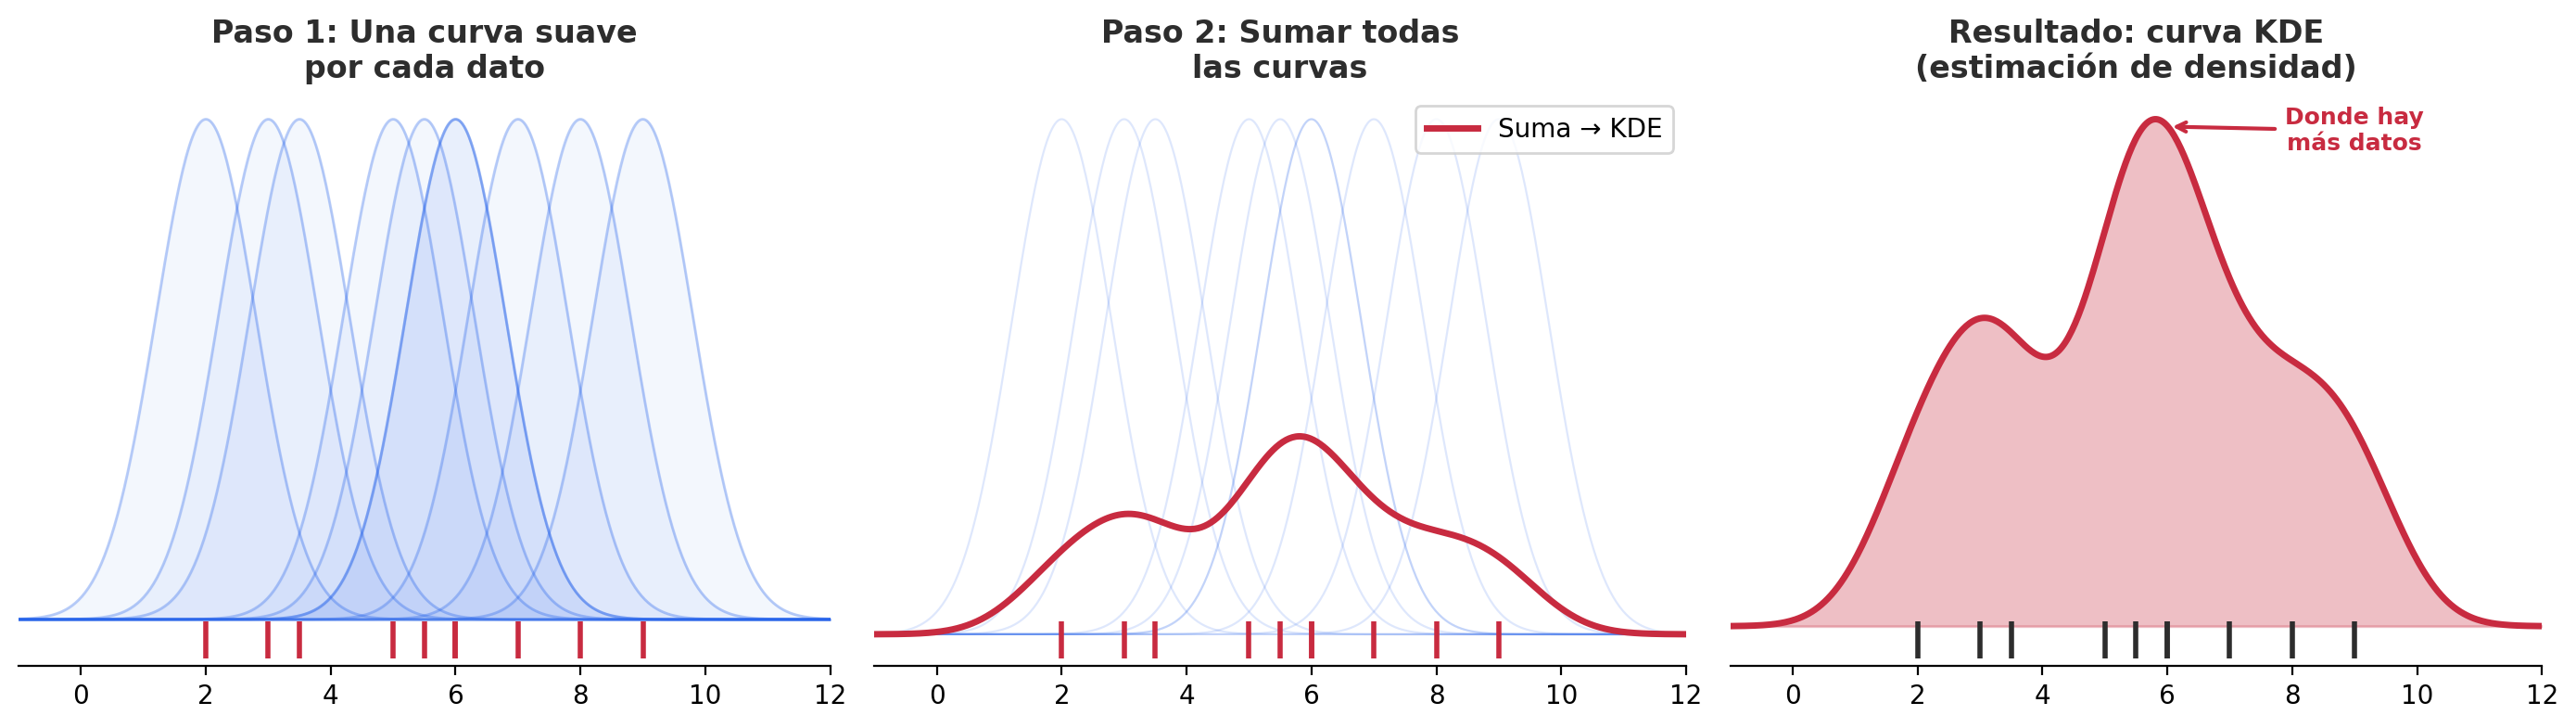
\includegraphics[width=\textwidth]{kde_explained.png}
  \end{center}

  \vspace{2pt}
  {\scriptsize\color{textMuted}
  \begin{itemize}\setlength{\itemsep}{3pt}
    \item[{\color{codeBlue}\scriptsize\faArrowRight}]
      \textbf{Paso 1:} Cada dato genera una pequeña curva centrada en su valor.
    \item[{\color{arcaRed}\scriptsize\faArrowRight}]
      \textbf{Paso 2:} Se suman todas las curvas y se promedian $\to$ una sola curva suave.
    \item[{\color{codeGreen}\scriptsize\faArrowRight}]
      \textbf{Resultado:} Donde hay más datos, la curva sube. Donde hay pocos, baja.
    \item[{\color{textMuted}\scriptsize\faLightbulb}]
      No necesitas memorizar la fórmula. Solo entiende: KDE = \textbf{versión suave del histograma}.
  \end{itemize}
  }
\end{frame}

\begin{frame}{Formas de Distribución}
  \vspace{-4pt}
  \begin{center}
    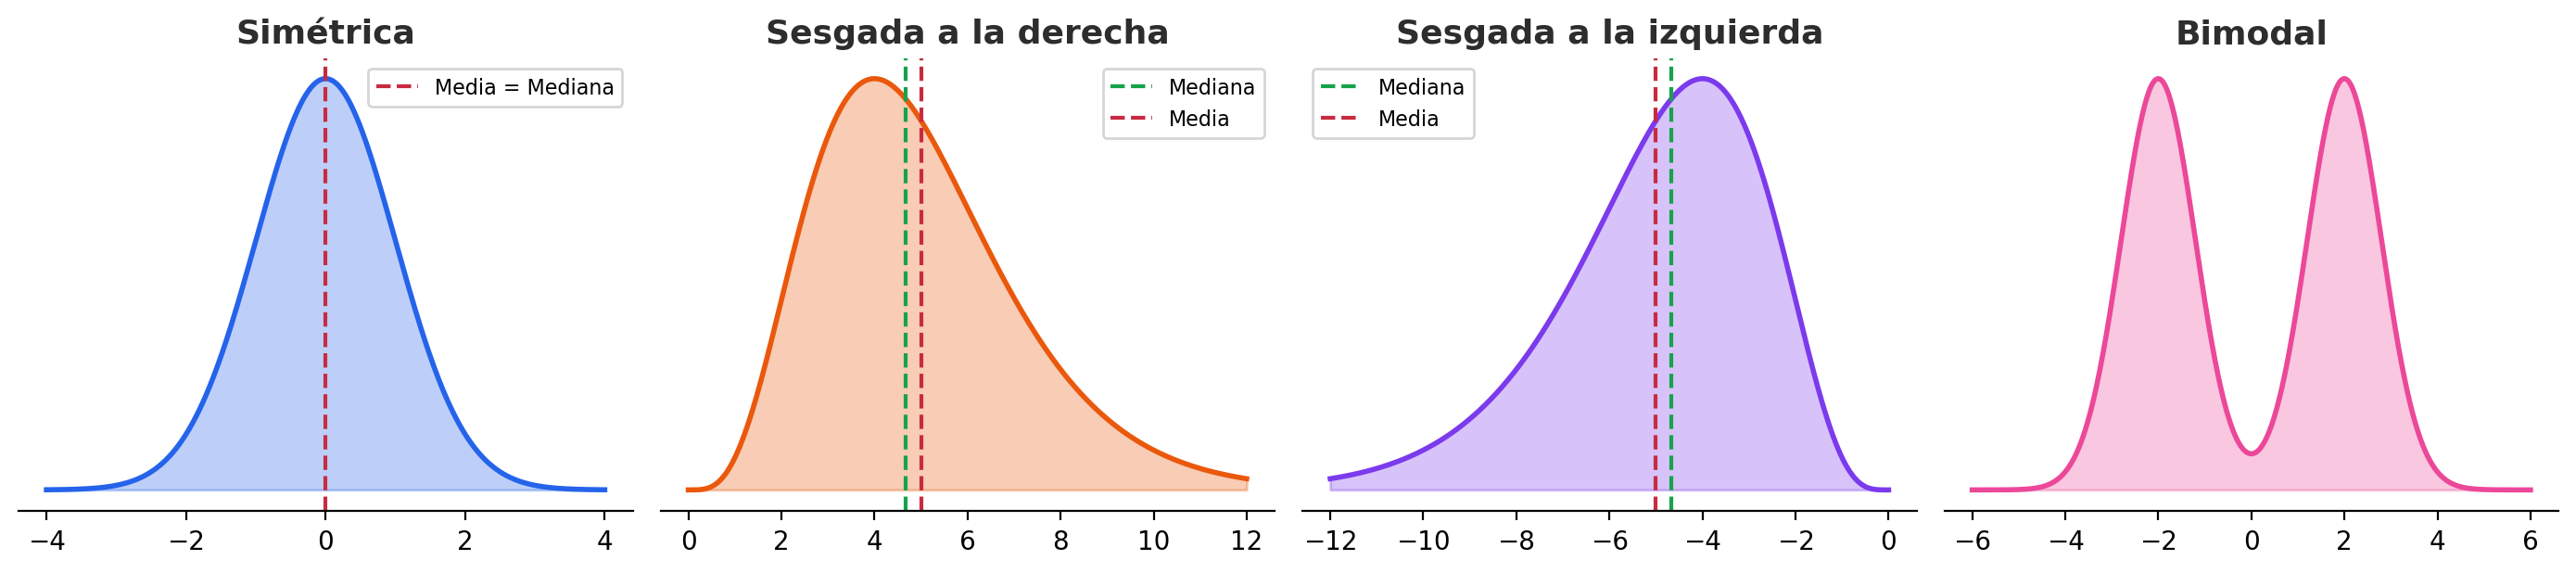
\includegraphics[width=\textwidth]{dist_shapes.png}
  \end{center}

  \vspace{4pt}
  {\scriptsize
  \begin{tabular}{@{}lll@{}}
    \toprule
    \textbf{Forma} & \textbf{Ejemplo en datos reales} & \textbf{Qué medida usar} \\
    \midrule
    Simétrica & Rating, estaturas, temperaturas & Media $\approx$ Mediana \\
    Sesgada derecha & Salarios, montos de venta, tiempos de espera & \textbf{Mediana} \\
    Sesgada izquierda & Edad de jubilación, notas de examen fácil & \textbf{Mediana} \\
    Bimodal & Mezcla de 2 poblaciones (hombre/mujer) & Separar y analizar cada grupo \\
    \bottomrule
  \end{tabular}
  }

  \vspace{4pt}
  {\scriptsize\color{textMuted}
    \faExclamationTriangle\ \textbf{Regla de oro:} Si la distribución es sesgada, la media \textbf{miente}.
    Usa la mediana.}
\end{frame}

\begin{frame}[shrink=5]{¿Por Qué Necesitamos Medir la Forma con Números?}
  \vspace{-4pt}
  {\footnotesize
    El histograma nos da una \textbf{imagen}, pero no un \textbf{número}.
    Sin un número no podemos comparar, automatizar, ni decidir con reglas claras.}

  \vspace{6pt}
  {\small
  \renewcommand{\arraystretch}{1.3}
  \begin{tabular}{@{}p{4cm}p{8.5cm}@{}}
    \toprule
    \textbf{Solo con el histograma} & \textbf{Con una medida numérica (skew)} \\
    \midrule
    ``Se ve medio sesgado\ldots'' &
      \texttt{skew = 1.42}: sesgo fuerte a la derecha $\to$ \textbf{usar mediana}. \\
    ``¿Será simétrico?'' &
      \texttt{skew = -0.08}: prácticamente simétrica $\to$ \textbf{media es confiable}. \\
    No puedes poner una imagen en un \texttt{if} &
      \texttt{if abs(skew) > 1: usar\_mediana()} $\to$ \textbf{automatizable}. \\
    Dos personas ``ven'' cosas distintas &
      El número es \textbf{objetivo y reproducible}. \\
    \bottomrule
  \end{tabular}
  }

  \vspace{6pt}
  {\scriptsize\color{textMuted}
    \faArrowRight\ El histograma es \textbf{el primer paso} (visual).
    Las medidas numéricas son \textbf{el segundo paso}: confirman, cuantifican y permiten decidir.}
\end{frame}

\begin{frame}[shrink=10]{La Forma Determina Tus Herramientas}
  \vspace{-4pt}
  {\footnotesize
    La forma de la distribución determina \textbf{qué herramientas usar}
    y \textbf{qué conclusiones son válidas}:}

  \vspace{6pt}
  {\small
  \renewcommand{\arraystretch}{1.3}
  \begin{tabular}{@{}p{3.2cm}p{4.3cm}p{4.3cm}@{}}
    \toprule
    \textbf{Decisión} & \textbf{Si es simétrica} & \textbf{Si es sesgada} \\
    \midrule
    ¿Qué promedio usar? &
      Media (confiable) &
      \textbf{Mediana} (la media miente) \\
    ¿Cómo medir dispersión? &
      Desviación estándar &
      \textbf{IQR} (robusta) \\
    ¿Cómo detectar outliers? &
      Z-score funciona bien &
      \textbf{Método IQR} \\
    ¿Cómo rellenar NaN? &
      Media &
      \textbf{Mediana} \\
    \bottomrule
  \end{tabular}
  }

  \vspace{6pt}
  {\scriptsize\color{textMuted}
    \faExclamationTriangle\ \textbf{Por eso lo primero es mirar la distribución:}
    si no sabes la forma, puedes elegir la herramienta equivocada y sacar conclusiones falsas.}
\end{frame}

\begin{frame}[shrink=15]{Sesgo (Skewness): La Fórmula}
  \vspace{-4pt}
  {\footnotesize
    El sesgo mide \textbf{cuánto y hacia dónde} se desvía la distribución de la simetría.}

  \vspace{6pt}
  \begin{center}
  \begin{tikzpicture}
    \node[rectangle, rounded corners=4pt, draw=arcaRed, fill=arcaRed!6,
          inner sep=10pt, font=\large\color{arcaDark}]
      {$\displaystyle g_1 = \frac{1}{n} \sum_{i=1}^{n} \left(\frac{x_i - \bar{x}}{s}\right)^{\!3}$};
  \end{tikzpicture}
  \end{center}

  \vspace{4pt}
  {\scriptsize
  \begin{tabular}{@{}cl@{}}
    \toprule
    \textbf{Símbolo} & \textbf{Significado} \\
    \midrule
    $n$ & Número total de observaciones (filas del dataset). \\
    $x_i$ & Cada observación individual ($x_1, x_2, \ldots, x_n$). \\
    $\bar{x}$ & La \textbf{media} aritmética: $\bar{x} = \frac{1}{n}\sum x_i$. \\
    $s$ & La \textbf{desviación estándar} (cuánto se dispersan los datos). \\
    $\frac{x_i - \bar{x}}{s}$ & Distancia de cada dato a la media, normalizada (z-score). \\
    $(\cdot)^3$ & Al elevar al cubo, se \textbf{preserva el signo}: valores a la derecha suman positivo, a la izquierda negativo. \\
    $\sum$ & Suma todos los valores desde $i=1$ hasta $n$. \\
    \bottomrule
  \end{tabular}
  }

  \vspace{4pt}
  {\scriptsize\color{textMuted}
    \faLightbulb\ ¿Por qué al \textbf{cubo}?
    Si fuera al cuadrado, los signos se cancelarían (como en la varianza).
    El cubo preserva si el dato está a la izquierda ($-$) o a la derecha ($+$) de la media.}
\end{frame}

\begin{frame}[fragile,shrink=28]{Sesgo en la Práctica}
  \vspace{-6pt}
  \begin{pyblock}
print("Sesgo de Rating:", df["Rating"].skew().round(3))
print("Sesgo de Total: ", df["Total"].skew().round(3))
  \end{pyblock}

  \vspace{4pt}
  \begin{center}
  \begin{tikzpicture}[
    box/.style={rectangle, rounded corners=3pt, draw=#1, fill=#1!8,
                minimum height=0.7cm, font=\scriptsize\bfseries, align=center},
  ]
    \node[box=codeGreen, minimum width=3cm] (sym) at (0,0)
      {\color{codeGreen}$-0.5 < \text{skew} < 0.5$\\Aprox. simétrica};
    \node[box=codeOrange, minimum width=3cm] (mod) at (5,0)
      {\color{codeOrange}$0.5 < |\text{skew}| < 1$\\Sesgo moderado};
    \node[box=arcaRed, minimum width=3cm] (high) at (10,0)
      {\color{arcaRed}$|\text{skew}| > 1$\\Sesgo fuerte};
  \end{tikzpicture}
  \end{center}

  \vspace{4pt}
  {\scriptsize\color{textMuted}
  \begin{itemize}\setlength{\itemsep}{3pt}
    \item[{\color{arcaRed}\scriptsize\faArrowRight}]
      \texttt{skew() > 0}: cola larga a la \textbf{derecha} (media > mediana).
    \item[{\color{arcaRed}\scriptsize\faArrowRight}]
      \texttt{skew() < 0}: cola larga a la \textbf{izquierda} (media < mediana).
    \item[{\color{arcaRed}\scriptsize\faArrowRight}]
      \texttt{skew() $\approx$ 0}: distribución \textbf{simétrica} (media $\approx$ mediana).
  \end{itemize}
  }
\end{frame}

% =============================================================================
%  SECCIÓN 2: TENDENCIA CENTRAL EN PROFUNDIDAD
% =============================================================================
\sectionframe{Tendencia Central}{Media, mediana y moda --- ahora en profundidad}

\begin{frame}[shrink=5]{¿Qué Buscamos Cuando Calculamos el ``Centro''?}
  \vspace{-4pt}
  {\footnotesize
    Cuando tenemos 1,000 transacciones, no podemos mirar una por una.
    Necesitamos \textbf{un solo número} que represente al grupo: la \textbf{tendencia central}.}

  \vspace{6pt}
  {\footnotesize
    Pero no existe un solo ``centro'' correcto. Depende de los datos y de la \textbf{pregunta que hagamos}:}

  \vspace{4pt}
  \begin{center}
  \begin{tikzpicture}[
    q/.style={rectangle, rounded corners=3pt, draw=arcaRed, fill=arcaRed!6,
              minimum width=5cm, minimum height=0.9cm,
              font=\scriptsize\color{textDark}, align=center, text width=4.6cm},
    a/.style={rectangle, rounded corners=3pt, draw=#1, fill=#1!8,
              minimum width=5cm, minimum height=0.9cm,
              font=\scriptsize\color{textDark}, align=center, text width=4.6cm},
  ]
    \node[q] (q1) at (0, 0)
      {``¿Cuánto \textbf{debería presupuestar}\\por transacción?''};
    \node[q] (q2) at (6.5, 0)
      {``¿Cuál es la experiencia\\de un \textbf{cliente típico}?''};
    \node[a=codeBlue, below=0.3cm of q1]
      {\textbf{Media}: reparte el total\\equitativamente entre todos};
    \node[a=codeGreen, below=0.3cm of q2]
      {\textbf{Mediana}: el valor que deja\\la mitad arriba y la mitad abajo};
  \end{tikzpicture}
  \end{center}

  \vspace{6pt}
  {\scriptsize\color{textMuted}
  \begin{itemize}\setlength{\itemsep}{3pt}
    \item[{\color{arcaRed}\scriptsize\faArrowRight}]
      La pregunta que haces determina qué medida usar.
      \textbf{No es que una sea mejor que la otra} --- responden preguntas distintas.
    \item[{\color{codeOrange}\scriptsize\faExclamationTriangle}]
      Si media y mediana \textbf{difieren mucho}, los datos tienen sesgo u outliers, y la media puede engañar.
  \end{itemize}
  }
\end{frame}

\begin{frame}[shrink=8]{¿Para Qué Usamos Media, Mediana y Moda?}
  \vspace{-4pt}
  {\scriptsize
  \begin{tabular}{@{}p{1.6cm}p{3cm}p{4cm}p{4cm}@{}}
    \toprule
    \textbf{Medida} & \textbf{¿Qué pregunta responde?} & \textbf{¿Qué información nos da?} & \textbf{Ejemplo en Arca} \\
    \midrule
    \textbf{Media} &
      ``Si repartiera el total entre todos, ¿cuánto le toca a cada uno?'' &
      Útil para \textbf{presupuestos y proyecciones}: media $\times$ N = total esperado.
      Funciona cuando los datos son \textbf{simétricos}. &
      ``El ingreso promedio por transacción es \$322'' $\to$ puedo proyectar ingresos mensuales. \\[4pt]
    \textbf{Mediana} &
      ``¿Cuál es la experiencia \textbf{típica} real?'' &
      Es lo que vive un cliente normal. \textbf{Inmune} a valores extremos.
      La mitad está arriba y la mitad abajo. &
      ``La venta típica es \$254'' $\to$ esto representa al cliente real, no un número inflado por compras gigantes. \\[4pt]
    \textbf{Moda} &
      ``¿Qué es lo más \textbf{popular}?'' &
      Preferencia y frecuencia. Única medida que funciona con \textbf{texto}. &
      ``El método de pago más usado es Ewallet'' $\to$ priorizar qué métodos soportar. \\
    \bottomrule
  \end{tabular}
  }

  \vspace{4pt}
  {\scriptsize\color{textMuted}
    \faLightbulb\ \textbf{Siempre calcula ambas} (media y mediana).
    Si coinciden $\to$ distribución simétrica, puedes usar cualquiera.
    Si difieren $\to$ hay sesgo, y la mediana es más confiable para comunicar ``lo típico''.}
\end{frame}

\begin{frame}[shrink=10]{La Media Aritmética: La Fórmula}
  \vspace{-4pt}
  \begin{center}
  \begin{tikzpicture}
    \node[rectangle, rounded corners=4pt, draw=codeBlue, fill=codeBlue!6,
          inner sep=10pt, font=\large\color{arcaDark}]
      {$\displaystyle \bar{x} = \frac{1}{n} \sum_{i=1}^{n} x_i = \frac{x_1 + x_2 + \cdots + x_n}{n}$};
  \end{tikzpicture}
  \end{center}

  \vspace{4pt}
  {\scriptsize
  \begin{tabular}{@{}cl@{}}
    \toprule
    \textbf{Símbolo} & \textbf{Significado} \\
    \midrule
    $\bar{x}$ & La media (se lee ``x barra''). Es el resultado. \\
    $x_i$ & Cada dato individual. El subíndice $i$ identifica cuál ($x_1$ = primer dato, $x_2$ = segundo\ldots). \\
    $n$ & Cantidad total de datos. \\
    $\sum_{i=1}^{n}$ & ``Suma desde $i=1$ hasta $n$''. Es decir, suma \textbf{todos} los datos. \\
    $\frac{\cdot}{n}$ & Dividir entre la cantidad de datos = \textbf{promedio}. \\
    \bottomrule
  \end{tabular}
  }

  \vspace{6pt}
  {\footnotesize\color{textDark}
    \textbf{Ejemplo:} Datos = \{4, 8, 6, 10, 2\}. \quad
    $\bar{x} = \frac{4+8+6+10+2}{5} = \frac{30}{5} = 6$}

  \vspace{4pt}
  {\scriptsize\color{textMuted}
    \faLightbulb\ En pandas: \texttt{df["col"].mean()} calcula esto automáticamente.}
\end{frame}

\begin{frame}[shrink=5]{Las Tres Medidas de Tendencia Central}
  \vspace{-4pt}
  \begin{center}
  \begin{tikzpicture}[
    scale=0.85, transform shape,
    card/.style={rectangle, rounded corners=4pt, draw=#1, fill=#1!6,
                 minimum width=4.5cm, minimum height=3.6cm, align=center},
    ttl/.style={font=\normalsize\bfseries\color{#1}},
    desc/.style={font=\tiny\color{textDark}, text width=3.8cm, align=left},
  ]
    \node[card=codeBlue] (med) at (0,0) {};
    \node[ttl=codeBlue, above] at (0, 0.9) {Media (\(\bar{x}\))};
    \node[desc] at (0, -0.1) {%
      Suma todos y divide entre $n$.\\[3pt]
      \textbf{Sirve para:} Presupuestos.\\
      media $\times$ N = total esperado.\\[2pt]
      \textbf{Pros:} Usa todos los datos.\\[2pt]
      \textbf{Contras:} Sensible a outliers.\\[2pt]
      \textbf{Código:} \texttt{df["col"].mean()}};

    \node[card=codeGreen] (mdn) at (5.5,0) {};
    \node[ttl=codeGreen, above] at (5.5, 0.9) {Mediana};
    \node[desc] at (5.5, -0.1) {%
      Ordena los datos y toma\\el valor del \textbf{medio}.\\[3pt]
      \textbf{Sirve para:} Saber la experiencia\\
      \textbf{típica real} de un cliente.\\[2pt]
      \textbf{Pros:} Robusta a outliers.\\[2pt]
      \textbf{Código:} \texttt{df["col"].median()}};

    \node[card=codeOrange] (mod) at (11,0) {};
    \node[ttl=codeOrange, above] at (11, 0.9) {Moda};
    \node[desc] at (11, -0.1) {%
      El valor que \textbf{más se repite}.\\[3pt]
      \textbf{Sirve para:} Saber lo más\\
      \textbf{popular} (preferencia, frecuencia).\\[2pt]
      \textbf{Pros:} Funciona con texto.\\[2pt]
      \textbf{Código:} \texttt{df["col"].mode()[0]}};
  \end{tikzpicture}
  \end{center}

  \vspace{4pt}
  {\scriptsize\color{textMuted}
    \faArrowRight\ \textbf{Ejemplo con \{2, 4, 4, 6, 100\}:}
    Media = 23.2 (inflada por el 100), Mediana = 4 (la experiencia real), Moda = 4 (lo más repetido).}
\end{frame}

\begin{frame}{Cuándo la Media Miente}
  \vspace{-4pt}
  \begin{center}
    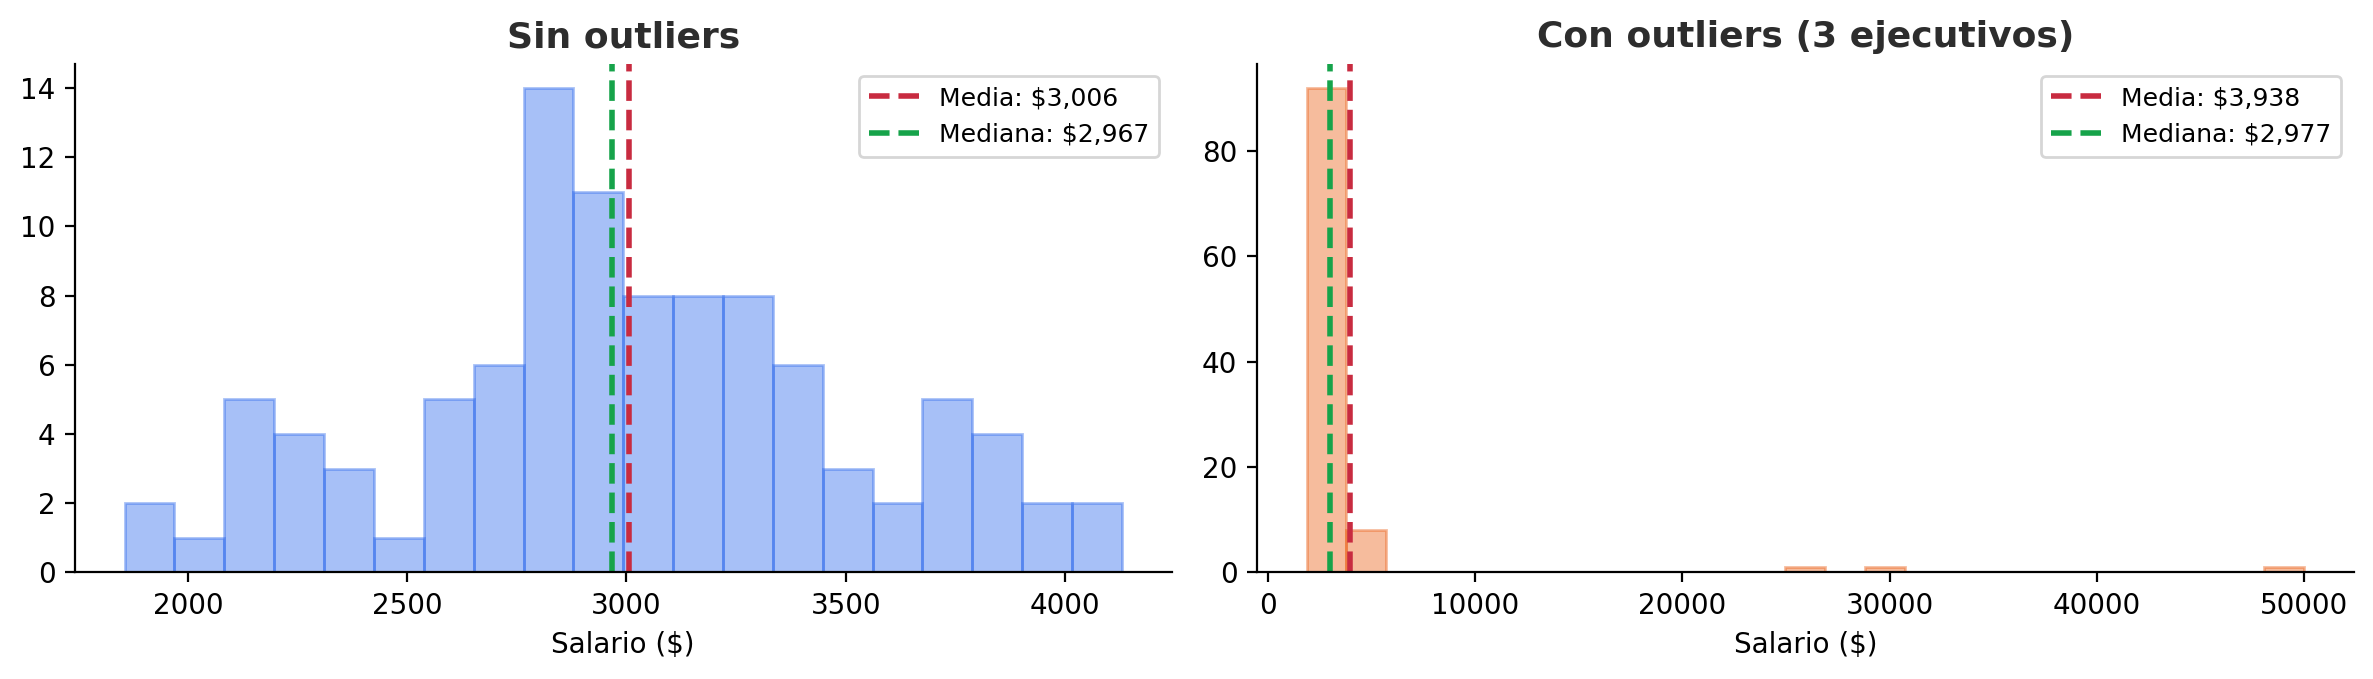
\includegraphics[width=0.95\textwidth]{mean_vs_median.png}
  \end{center}

  \vspace{4pt}
  {\scriptsize\color{textMuted}
  \begin{itemize}\setlength{\itemsep}{3pt}
    \item[{\color{codeOrange}\scriptsize\faExclamationTriangle}]
      3 ejecutivos con salarios altos \textbf{arrastraron la media} hacia arriba.
    \item[{\color{codeGreen}\scriptsize\faCheckCircle}]
      La mediana \textbf{apenas se movió} --- es robusta a valores extremos.
    \item[{\color{arcaRed}\scriptsize\faArrowRight}]
      Siempre compara media vs mediana. Si difieren mucho, hay \textbf{sesgo u outliers}.
  \end{itemize}
  }
\end{frame}

\begin{frame}[fragile,shrink=28]{Tendencia Central en Nuestro Dataset}
  \vspace{-6pt}
  \begin{pyblock}
cols_num = ["Total", "Rating", "gross income", "Tax 5%"]
for col in cols_num:
    s = df[col].dropna()
    print(f"{col:>15}  |  media={s.mean():8.2f}  "
          f"mediana={s.median():8.2f}  "
          f"diff={abs(s.mean()-s.median()):6.2f}")
  \end{pyblock}

  \vspace{4pt}
  {\scriptsize\color{textMuted}
  \begin{itemize}\setlength{\itemsep}{3pt}
    \item[{\color{arcaRed}\scriptsize\faArrowRight}]
      Si \texttt{diff} es grande $\to$ distribución sesgada $\to$ preferir mediana.
    \item[{\color{arcaRed}\scriptsize\faArrowRight}]
      Si \texttt{diff} es pequeña $\to$ distribución simétrica $\to$ la media es confiable.
  \end{itemize}
  }
\end{frame}

\begin{frame}[fragile,shrink=28]{Visualizar Media vs Mediana sobre el Histograma}
  \vspace{-6pt}
  \begin{pyblock}
data = df["Total"].dropna()

sns.histplot(data, kde=True, bins=30, color="#2563EB",
             alpha=0.4)
plt.axvline(data.mean(), color="#C82B40", linestyle="--",
            linewidth=2, label=f"Media: {data.mean():.1f}")
plt.axvline(data.median(), color="#16A34A", linestyle="--",
            linewidth=2, label=f"Mediana: {data.median():.1f}")
plt.legend(fontsize=11)
plt.title("Distribucion de Total")
plt.show()
  \end{pyblock}

  \vspace{4pt}
  {\scriptsize\color{textMuted}
    \faLightbulb\ \texttt{plt.axvline()} dibuja una línea vertical --- ideal para marcar estadísticos sobre un gráfico.}
\end{frame}

% =============================================================================
%  SECCIÓN 3: MEDIDAS DE DISPERSIÓN
% =============================================================================
\sectionframe{Medidas de Dispersión}{¿Qué tan dispersos están los datos?}

\begin{frame}{¿Por Qué Importa la Dispersión?}
  \vspace{-4pt}
  \begin{center}
  \begin{tikzpicture}[
    box/.style={rectangle, rounded corners=4pt, draw=#1, fill=#1!8,
                minimum width=5.5cm, minimum height=2.5cm,
                font=\scriptsize\color{textDark}, align=center, text width=5cm},
  ]
    \node[box=codeBlue] (a) at (0,0) {%
      \textbf{\color{codeBlue}\normalsize Grupo A}\\[4pt]
      Salarios: \$3000, \$3100, \$2900,\\
      \$3050, \$2950\\[4pt]
      Media = \$3000\\
      \textbf{Todos ganan parecido}};
    \node[box=codeOrange] (b) at (7,0) {%
      \textbf{\color{codeOrange}\normalsize Grupo B}\\[4pt]
      Salarios: \$500, \$1000, \$3000,\\
      \$5000, \$5500\\[4pt]
      Media = \$3000\\
      \textbf{Enorme desigualdad}};

    \node[font=\Large\bfseries\color{arcaRed}] at (3.5, 0) {$\neq$};
  \end{tikzpicture}
  \end{center}

  \vspace{6pt}
  {\footnotesize\color{textMuted}
    \faExclamationTriangle\ \textbf{Misma media, realidades totalmente distintas.}
    La dispersión completa la historia que la media no cuenta.}
\end{frame}

\begin{frame}[shrink=15]{Varianza y Desviación Estándar: La Fórmula Paso a Paso}
  \vspace{-4pt}
  {\footnotesize
    Queremos medir: \textbf{en promedio, qué tan lejos está cada dato de la media.}}

  \vspace{4pt}
  \begin{center}
  \begin{tikzpicture}
    \node[rectangle, rounded corners=4pt, draw=codeBlue, fill=codeBlue!6,
          inner sep=10pt, font=\large\color{arcaDark}]
      {$\displaystyle s^2 = \frac{1}{n-1} \sum_{i=1}^{n} (x_i - \bar{x})^2
       \qquad\qquad s = \sqrt{s^2}$};
  \end{tikzpicture}
  \end{center}

  \vspace{4pt}
  {\scriptsize
  \begin{tabular}{@{}lll@{}}
    \toprule
    \textbf{Paso} & \textbf{Qué hacemos} & \textbf{¿Por qué?} \\
    \midrule
    $x_i - \bar{x}$ & Distancia de cada dato a la media & Para saber cuánto se aleja cada uno \\
    $(x_i - \bar{x})^2$ & Elevamos al cuadrado & Para que todas sean \textbf{positivas} (si no, se cancelan) \\
    $\sum$ & Sumamos todas & Para acumular la dispersión total \\
    $\div\;(n-1)$ & Dividimos entre $n{-}1$ & Para obtener un \textbf{promedio} de dispersión \\
    $\sqrt{\phantom{x}}$ & Raíz cuadrada & Para volver a las \textbf{unidades originales} (de \$\textsuperscript{2} a \$) \\
    \bottomrule
  \end{tabular}
  }

  \vspace{4pt}
  {\footnotesize\color{textDark}
    \textbf{Ejemplo:} Datos = \{2, 4, 4, 4, 5, 5, 7, 9\}. \quad $\bar{x} = 5$.\\[2pt]
    Distancias$^2$: $(2{-}5)^2 + (4{-}5)^2 + \cdots + (9{-}5)^2 = 9+1+1+1+0+0+4+16 = 32$\\[2pt]
    $s^2 = \frac{32}{7} = 4.57$ \qquad $s = \sqrt{4.57} = 2.14$\\[2pt]
    \textbf{Interpretación:} ``En promedio, los datos se alejan \textbf{2.14 unidades} de la media.''}

  \vspace{3pt}
  {\scriptsize\color{textMuted}
    \faLightbulb\ En pandas: \texttt{.var()} calcula $s^2$ y \texttt{.std()} calcula $s$ (ambas usan $n-1$).}
\end{frame}

\begin{frame}[shrink=10]{Varianza vs Desviación Estándar: Qué Nos Dicen y Cuándo Usar Cada Una}
  \vspace{-4pt}
  {\footnotesize
    Ambas miden \textbf{la misma idea}: qué tan lejos están los datos de la media.
    La diferencia es \textbf{la unidad} y \textbf{para qué las lees}.}

  \vspace{6pt}
  {\scriptsize
  \begin{tabular}{@{}p{2.8cm}p{5.2cm}p{5.5cm}@{}}
    \toprule
    \textbf{Medida} & \textbf{Qué información te da} & \textbf{Cuándo usarla} \\
    \midrule
    \textbf{Varianza} ($s^2$) &
      Dispersión en \textbf{unidades al cuadrado} (ej.\ dólares$^2$, estrellas$^2$).
      Es difícil de interpretar ``en la cabeza'', pero matemáticamente útil. &
      En \textbf{fórmulas} y modelos (regresión, ANOVA, algunos algoritmos) donde se suman varianzas o se optimiza error cuadrático.
      Para \textbf{reportar a negocio}, casi nunca. \\
    \textbf{Desv.\ estándar} ($s$) &
      ``En promedio, los datos se alejan unos \textbf{$s$ unidades} de la media.''
      Misma escala que los datos $\to$ \textbf{interpretable}. &
      Reportes, gráficos, Z-score, comparar dispersión \textbf{dentro de la misma variable} en el tiempo o entre grupos con la misma unidad. \\
    \bottomrule
  \end{tabular}
  }

  \vspace{6pt}
  {\scriptsize\color{textMuted}
  \begin{itemize}\setlength{\itemsep}{3pt}
    \item[{\color{codeGreen}\scriptsize\faCheckCircle}]
      \textbf{Regla simple:} Comunica con \texttt{.std()}; usa \texttt{.var()} cuando el código o la teoría lo pida.
    \item[{\color{codeOrange}\scriptsize\faExclamationTriangle}]
      Std (como la media) es \textbf{sensible a outliers}. Si la distribución es muy sesgada, complementa con \textbf{IQR}.
  \end{itemize}
  }
\end{frame}

\begin{frame}[shrink=10]{Cuartiles: Dividir los Datos en 4 Partes Iguales}
  \vspace{-4pt}
  {\footnotesize
    Imagina que \textbf{ordenas todos} los datos de menor a mayor y los cortas en \textbf{4 partes iguales} (como un pastel).
    Los puntos donde cortas se llaman \textbf{cuartiles}:}

  \vspace{4pt}
  \begin{center}
  \begin{tikzpicture}[
    seg/.style={rectangle, minimum height=1cm, fill=#1!20, draw=#1!60,
                font=\scriptsize\bfseries\color{#1!80!black}, align=center},
    lbl/.style={font=\scriptsize\bfseries\color{arcaRed}},
  ]
    \node[seg=codeBlue, minimum width=3cm] (s1) at (0, 0)     {25\% más\\bajos};
    \node[seg=codeGreen, minimum width=3cm] (s2) at (3.1, 0)  {Siguiente\\25\%};
    \node[seg=codeGreen, minimum width=3cm] (s3) at (6.2, 0)  {Siguiente\\25\%};
    \node[seg=codeOrange, minimum width=3cm] (s4) at (9.3, 0) {25\% más\\altos};

    \node[lbl, below=0.15cm] at (s1.south east) {Q1};
    \node[lbl, below=0.15cm] at (s2.south east) {Q2 = Mediana};
    \node[lbl, below=0.15cm] at (s3.south east) {Q3};

    \draw[decorate, decoration={brace, amplitude=5pt, mirror}, arcaRed, thick]
      ([yshift=-0.8cm]s2.south west) -- ([yshift=-0.8cm]s3.south east)
      node[midway, below=6pt, font=\footnotesize\bfseries\color{arcaRed}] {IQR = Q3 $-$ Q1};
  \end{tikzpicture}
  \end{center}

  \vspace{4pt}
  {\scriptsize
  \begin{tabular}{@{}lll@{}}
    \toprule
    \textbf{Cuartil} & \textbf{Significado} & \textbf{Interpretación de negocio} \\
    \midrule
    \textbf{Q1} (percentil 25) & 25\% de los datos está \textbf{por debajo} & ``Las ventas bajas llegan hasta aquí'' \\
    \textbf{Q2} (percentil 50) & 50\% por debajo $=$ \textbf{la mediana} & ``La venta típica'' \\
    \textbf{Q3} (percentil 75) & 75\% de los datos está \textbf{por debajo} & ``Solo el 25\% supera este monto'' \\
    \bottomrule
  \end{tabular}
  }

  \vspace{4pt}
  {\scriptsize\color{textMuted}
    \faLightbulb\ En pandas: \texttt{df["col"].quantile(0.25)} para Q1, \texttt{.quantile(0.75)} para Q3.}
\end{frame}

\begin{frame}[shrink=15]{IQR: El Rango del 50\% Central}
  \vspace{-4pt}

  \begin{center}
  \begin{tikzpicture}
    \node[rectangle, rounded corners=4pt, draw=arcaRed, fill=arcaRed!6,
          inner sep=10pt, font=\large\color{arcaDark}]
      {$\text{IQR} = Q3 - Q1$};
  \end{tikzpicture}
  \end{center}

  \vspace{4pt}
  {\footnotesize
    El \textbf{IQR} (Rango Intercuartílico) mide \textbf{qué tan ancho es el rango del 50\% central} de los datos.
    Ignora el 25\% más bajo y el 25\% más alto.}

  \vspace{4pt}
  {\scriptsize
    \textbf{Ejemplo paso a paso:} Datos = \{12, 15, 18, 22, 25, 30, 35, 50\}\\[2pt]
    1.~Ordenar (ya están).\\
    2.~Q2 (mediana): promedio del 4to y 5to = $(22+25)/2 = 23.5$\\
    3.~Q1: mediana de \{12, 15, 18, 22\} = $(15+18)/2 = 16.5$\\
    4.~Q3: mediana de \{25, 30, 35, 50\} = $(30+35)/2 = 32.5$\\
    5.~\textbf{IQR} $= 32.5 - 16.5 = 16$}

  \vspace{6pt}
  {\scriptsize
  \begin{tabular}{@{}lp{10cm}@{}}
    \toprule
    \textbf{¿Por qué es útil?} & \textbf{Explicación} \\
    \midrule
    \textbf{Robusta a outliers} & Como solo mira el 50\% central, un dato extremo no la afecta. Si alguien compra \$50,000, el IQR no cambia. \\[3pt]
    \textbf{Complementa la mediana} & Si usas la mediana como centro, usa el IQR como dispersión (las dos son robustas). \\[3pt]
    \textbf{Detecta outliers} & Es la base del método IQR: todo dato fuera de $[Q1 - 1.5 \times \text{IQR},\; Q3 + 1.5 \times \text{IQR}]$ es outlier potencial. \\
    \bottomrule
  \end{tabular}
  }

  \vspace{4pt}
  {\scriptsize\color{textMuted}
    \faArrowRight\ \textbf{Información:} ``El 50\% central de las ventas va de \$Q1 a \$Q3, un rango de \$IQR.''}
\end{frame}

\begin{frame}[shrink=25]{Las Medidas de Dispersión --- Resumen}
  \vspace{-4pt}
  {\small
  \begin{tabular}{@{}llp{4.5cm}ll@{}}
    \toprule
    \textbf{Medida} & \textbf{Fórmula} & \textbf{Interpretación} & \textbf{Código} & \textbf{¿Robusta?} \\
    \midrule
    Rango & $\max - \min$ &
      Diferencia entre extremos. Un solo outlier lo infla. &
      \texttt{.max()-.min()} & No \\[4pt]
    Varianza ($s^2$) & $\frac{\sum(x_i - \bar{x})^2}{n-1}$ &
      Dispersión promedio (en unidades$^2$). Para fórmulas. &
      \texttt{.var()} & No \\[4pt]
    Desv.\ estándar ($s$) & $\sqrt{s^2}$ &
      ``En promedio, los datos se alejan $s$ unidades de la media.'' &
      \texttt{.std()} & No \\[4pt]
    \textbf{IQR} & $Q3 - Q1$ &
      Ancho del 50\% central. &
      \texttt{.quantile(.75)}\newline\texttt{-.quantile(.25)} & \textbf{Sí} \\
    \bottomrule
  \end{tabular}
  }

  \vspace{6pt}
  {\scriptsize\color{textMuted}
  \begin{itemize}\setlength{\itemsep}{3pt}
    \item[{\color{codeGreen}\scriptsize\faCheckCircle}]
      \textbf{Distribución simétrica:} usa media + std (aprovechan todos los datos).
    \item[{\color{codeOrange}\scriptsize\faExclamationTriangle}]
      \textbf{Distribución sesgada / outliers:} usa mediana + IQR (robustas).
  \end{itemize}
  }
\end{frame}

\begin{frame}[fragile,shrink=28]{Dispersión en Código}
  \vspace{-6pt}
  \begin{pyblock}
col = "Total"
data = df[col].dropna()

rango = data.max() - data.min()
varianza = data.var()
std = data.std()
q1 = data.quantile(0.25)
q3 = data.quantile(0.75)
iqr = q3 - q1

print(f"Rango:     {rango:.2f}")
print(f"Varianza:  {varianza:.2f}")
print(f"Std:       {std:.2f}")
print(f"Q1={q1:.2f}, Q3={q3:.2f}, IQR={iqr:.2f}")
  \end{pyblock}

  \vspace{4pt}
  {\scriptsize\color{textMuted}
    \faLightbulb\ \texttt{df.describe()} muestra todo esto de una vez: count, mean, std, min, 25\%, 50\%, 75\%, max.}
\end{frame}

\begin{frame}[fragile,shrink=28]{\texttt{df.describe()}: El Resumen Completo}
  \vspace{-6pt}
  \begin{pyblock}
print(df[["Total", "Rating", "Quantity"]].describe().round(2))
  \end{pyblock}

  \vspace{2pt}
  \begin{outputblock}[minted options={fontsize=\scriptsize, breaklines}]
         Total   Rating  Quantity
count   985.00   965.00   1000.00
mean    322.50     6.97      5.51
std     245.89     1.72      2.77
min      10.68     4.00      1.00
25%     124.42     5.50      3.00
50%     253.85     7.00      5.00
75%     471.35     8.50      8.00
max    1042.65    10.00     10.00
  \end{outputblock}

  \vspace{4pt}
  {\scriptsize\color{textMuted}
    \faArrowRight\ Cada fila cuenta una historia: \texttt{count} revela NaN,
    \texttt{std} la dispersión, \texttt{50\%} es la mediana.}
\end{frame}

\begin{frame}[shrink=8]{Coeficiente de Variación (CV): Para Qué Sirve y Cuándo Usarlo}
  \vspace{-4pt}
  {\footnotesize
    La \textbf{std} y la \textbf{varianza} comparan dispersión cuando la \textbf{unidad es la misma}.
    El CV compara \textbf{dispersión relativa}: ``¿qué tan grande es la std \textit{respecto} a la media?''}

  \vspace{4pt}
  \begin{center}
  \begin{tikzpicture}[
    card/.style={rectangle, rounded corners=4pt, draw=arcaRed, fill=arcaRed!6,
                 minimum width=5cm, minimum height=1.0cm,
                 font=\normalsize\bfseries\color{arcaDark}, align=center},
  ]
    \node[card] (cv) at (0,0)
      {$\text{CV} = \dfrac{s}{|\bar{x}|} \times 100\%$};
  \end{tikzpicture}
  \end{center}

  \vspace{4pt}
  {\scriptsize
  \begin{tabular}{@{}p{3.2cm}p{9.5cm}@{}}
    \toprule
    \textbf{Cuándo usar CV} & \textbf{Ejemplos} \\
    \midrule
    Comparar \textbf{dos columnas} con unidades distintas &
      \texttt{Rating} (1--10) vs \texttt{Total} (dólares): la std de \texttt{Total} es enorme en número, pero no significa ``más caótico'' sin el CV. Con CV ves cuál es \textbf{más variable en proporción a su promedio}. \\
    Comparar \textbf{la misma métrica} entre sucursales o meses &
      ``¿En qué sucursal las ventas \textbf{oscilan más} en torno a su promedio?'' --- útil para priorizar dónde estabilizar procesos. \\
    \midrule
    \textbf{Cuándo NO usar CV} & Si $\bar{x} \approx 0$ o hay valores negativos mezclados, el CV pierde sentido o se vuelve engañoso. Ahí usa IQR o std en valor absoluto. \\
    \bottomrule
  \end{tabular}
  }

  \vspace{4pt}
  {\footnotesize
  \begin{itemize}\setlength{\itemsep}{3pt}
    \item[{\color{codeBlue}\scriptsize\faArrowRight}]
      \textbf{Rating:} std $\approx$ 1.7, media $\approx$ 7.0 $\to$ CV $\approx$ 24\%.
    \item[{\color{codeOrange}\scriptsize\faArrowRight}]
      \textbf{Total:} std $\approx$ 246, media $\approx$ 322 $\to$ CV $\approx$ 76\%.
    \item[{\color{arcaRed}\scriptsize\faArrowRight}]
      \textbf{Lectura:} \texttt{Total} es \textbf{más heterogéneo en términos relativos} que \texttt{Rating}.
  \end{itemize}
  }

  \vspace{2pt}
  {\scriptsize\color{textMuted}
    \faLightbulb\ CV alto (p.\ ej.\ $>$ 30--40\%) suele indicar mucha variabilidad \textbf{respecto al nivel típico}; el umbral depende del contexto del negocio.}
\end{frame}

% ── EJERCICIO 1 ──────────────────────────────────────────────────────────────
\begin{frame}[fragile,shrink=28]{Ejercicio 1: Explora la Distribución \hfill
    {\normalsize\color{arcaRed}\faClock\ 5 min}}
  \vspace{-6pt}
  {\footnotesize\color{arcaDark}\bfseries
    Sobre el dataset \texttt{df} que ya cargamos:}

  \vspace{4pt}
  \begin{pyblock}
# 1. Histograma + KDE de "Rating"
#    Pista: sns.histplot(df["Rating"].dropna(),
#           kde=True, bins=20)

# 2. Histograma + KDE de "Total"
#    Cual se ve mas simetrica?

# 3. Calcula media, mediana y skew de ambas

# 4. Cual tiene mayor CV?
#    Pista: (std / mean) * 100
  \end{pyblock}

  \vspace{4pt}
  {\scriptsize\color{textMuted}
  \begin{itemize}\setlength{\itemsep}{3pt}
    \item[{\color{arcaRed}\scriptsize\faLightbulb}]
      Si \texttt{skew} $\approx 0$ y media $\approx$ mediana $\to$ distribución simétrica.
    \item[{\color{arcaRed}\scriptsize\faLightbulb}]
      Si CV $>$ 30\% $\to$ alta dispersión relativa.
  \end{itemize}
  }
\end{frame}

% =============================================================================
%  SECCIÓN 4: OUTLIERS
% =============================================================================
\sectionframe{Outliers}{Detectar y decidir qué hacer con ellos}

\begin{frame}{¿Qué Es un Outlier?}
  \vspace{-4pt}
  \begin{center}
  \begin{tikzpicture}[
    box/.style={rectangle, rounded corners=4pt, draw=#1, fill=#1!8,
                minimum width=5cm, minimum height=1.5cm,
                font=\scriptsize\color{textDark}, align=center, text width=4.5cm},
  ]
    \node[box=codeOrange] (def) at (0,0)
      {\textbf{\color{codeOrange}\normalsize Outlier}\\[2pt]
       Dato que se aleja significativamente\\
       del resto de observaciones.};
    \node[box=codeGreen] (ok) at (6,0.8)
      {\textbf{\color{codeGreen}No siempre es error}\\[2pt]
       Una compra de \$1000 es legítima\\
       (un cliente que compró mucho).};
    \node[box=arcaRed] (bad) at (6,-0.8)
      {\textbf{\color{arcaRed}A veces sí es error}\\[2pt]
       Una edad de $-5$ años o un\\
       salario de \$0 son errores claros.};

    \draw[-{Stealth[length=3pt]}, line width=0.6pt, textMuted]
      (def.east) -- (ok.west);
    \draw[-{Stealth[length=3pt]}, line width=0.6pt, textMuted]
      (def.east) -- (bad.west);
  \end{tikzpicture}
  \end{center}

  \vspace{6pt}
  {\scriptsize\color{textMuted}
    \faExclamationTriangle\ \textbf{Nunca elimines outliers automáticamente.}
    Primero entiende \textit{por qué} el dato es extremo. El contexto de negocio decide.}
\end{frame}

\begin{frame}{Método IQR para Detectar Outliers}
  \vspace{-4pt}
  \begin{center}
    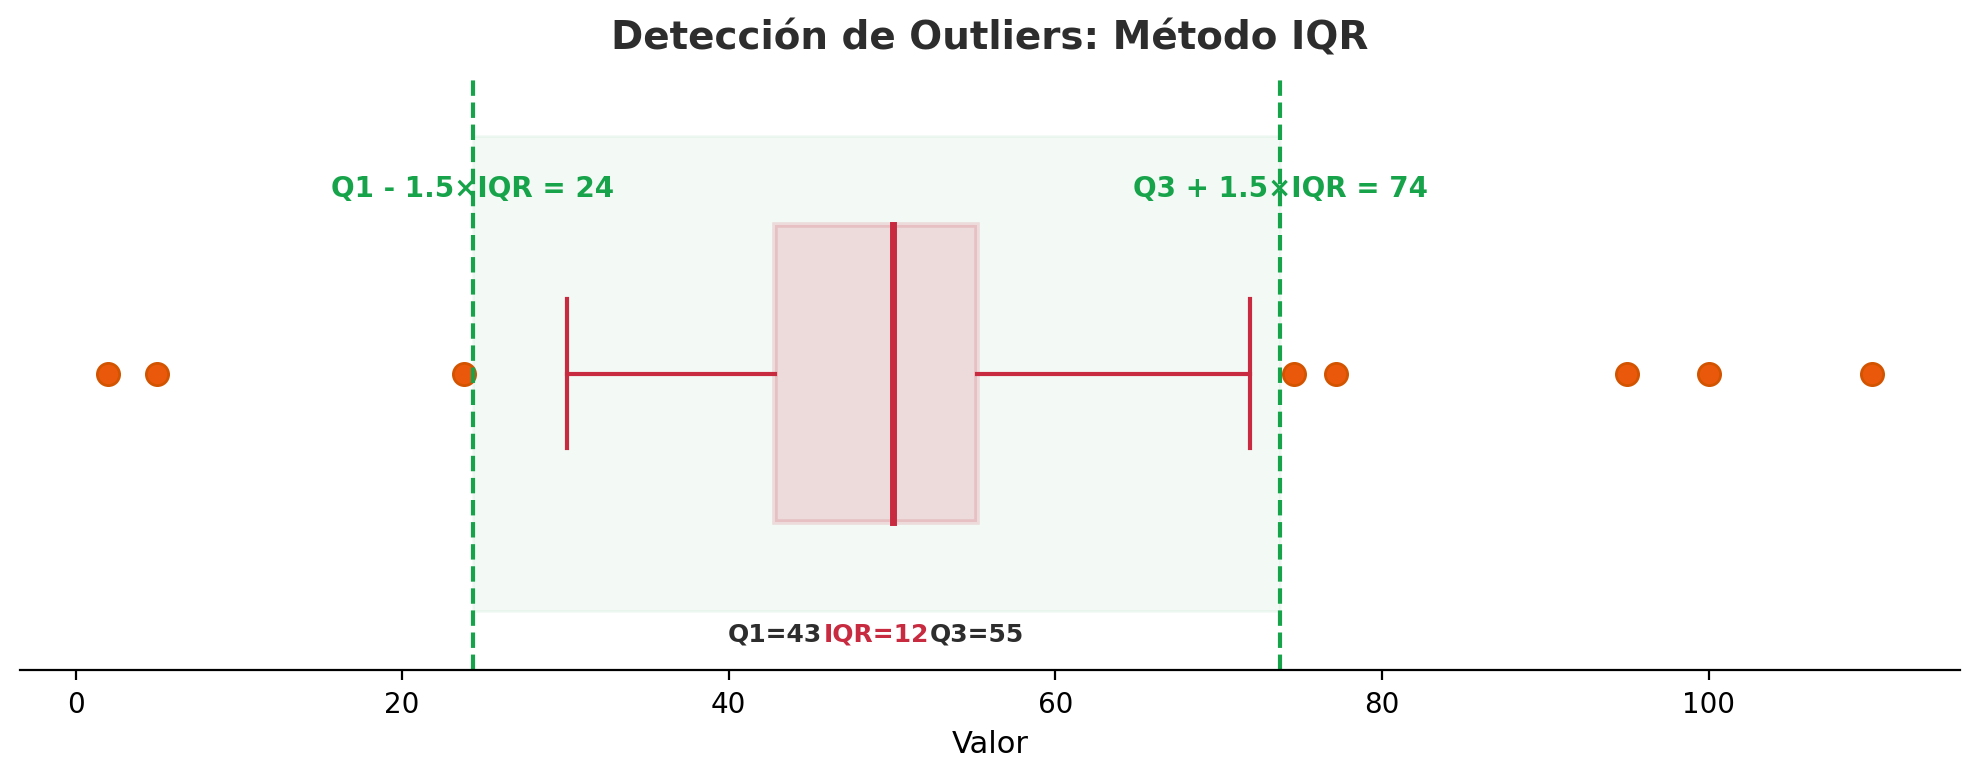
\includegraphics[width=0.9\textwidth]{outlier_iqr.png}
  \end{center}

  \vspace{4pt}
  {\scriptsize\color{textMuted}
  \begin{itemize}\setlength{\itemsep}{3pt}
    \item[{\color{arcaRed}\scriptsize\faArrowRight}]
      \textbf{Límite inferior:} $Q1 - 1.5 \times \text{IQR}$
    \item[{\color{arcaRed}\scriptsize\faArrowRight}]
      \textbf{Límite superior:} $Q3 + 1.5 \times \text{IQR}$
    \item[{\color{codeOrange}\scriptsize\faExclamationTriangle}]
      Todo dato fuera de estos límites se marca como \textbf{outlier potencial}.
  \end{itemize}
  }
\end{frame}

\begin{frame}[fragile,shrink=28]{Detectar Outliers en Código}
  \vspace{-6pt}
  \begin{pyblock}
col = "Total"
data = df[col].dropna()

q1 = data.quantile(0.25)
q3 = data.quantile(0.75)
iqr = q3 - q1

lim_inf = q1 - 1.5 * iqr
lim_sup = q3 + 1.5 * iqr

outliers = data[(data < lim_inf) | (data > lim_sup)]

print(f"Limites: [{lim_inf:.1f}, {lim_sup:.1f}]")
print(f"Outliers encontrados: {len(outliers)}")
print(f"Porcentaje: {len(outliers)/len(data)*100:.1f}%")
  \end{pyblock}

  \vspace{4pt}
  {\scriptsize\color{textMuted}
    \faLightbulb\ El operador \texttt{|} (``o'') combina dos condiciones booleanas.
    Filtramos datos menores al límite inferior O mayores al superior.}
\end{frame}

\begin{frame}[fragile,shrink=28]{Visualizar Outliers: Boxplot + Stripplot}
  \vspace{-6pt}
  \begin{pyblock}
sns.boxplot(data=df, x="Total",
            color="#C82B40", width=0.3)
sns.stripplot(data=df, x="Total",
              color="#2563EB", alpha=0.3, size=3)
plt.title("Total: Boxplot + puntos reales")
plt.show()
  \end{pyblock}

  \vspace{4pt}
  {\scriptsize\color{textMuted}
  \begin{itemize}\setlength{\itemsep}{3pt}
    \item[{\color{arcaRed}\scriptsize\faArrowRight}]
      \texttt{sns.stripplot()} muestra \textbf{cada punto individual} --- ves la densidad real.
    \item[{\color{arcaRed}\scriptsize\faArrowRight}]
      Los outliers del boxplot coinciden con los puntos aislados del stripplot.
  \end{itemize}
  }
\end{frame}

\begin{frame}{¿Eliminar o Conservar? Criterio de Negocio}
  \vspace{-4pt}
  {\small
  \begin{tabular}{@{}p{5cm}p{5cm}@{}}
    \toprule
    \textbf{\color{arcaRed}Eliminar cuando\ldots} &
    \textbf{\color{codeGreen}Conservar cuando\ldots} \\
    \midrule
    Es un error de registro\newline
    (edad negativa, precio \$0). &
    Es un dato real pero extremo\newline
    (cliente VIP, compra navideña). \\[8pt]
    Distorsiona el modelo\newline
    (regresión, clustering). &
    Es justamente lo que buscas\newline
    (detección de fraude). \\[8pt]
    El porcentaje es $<$ 1--2\%\newline
    y no afecta representatividad. &
    Representa un segmento real\newline
    que el negocio debe atender. \\
    \bottomrule
  \end{tabular}
  }

  \vspace{8pt}
  {\scriptsize\color{textMuted}
    \faArrowRight\ Alternativa: en lugar de eliminar, puedes \textbf{truncar} (winsorize)
    los valores extremos al percentil 1\% y 99\%.}
\end{frame}

% =============================================================================
%  SECCIÓN 5: DISTRIBUCIÓN NORMAL
% =============================================================================
\sectionframe{La Distribución Normal}{La campana más famosa de la estadística}

\begin{frame}[shrink=10]{¿Por Qué Importa la Normal?}
  \vspace{-4pt}
  \begin{center}
  \begin{tikzpicture}[
    box/.style={rectangle, rounded corners=4pt, draw=#1, fill=#1!8,
                minimum width=4.8cm, minimum height=1.8cm,
                font=\scriptsize\color{textDark}, align=center, text width=4.3cm},
  ]
    \node[box=codeBlue] (nat) at (0,0)
      {\textbf{\color{codeBlue}Aparece en la naturaleza}\\[2pt]
       Estaturas, pesos, errores\\
       de medición, IQ\ldots};
    \node[box=codeGreen] (math) at (5.5,0)
      {\textbf{\color{codeGreen}Base matemática}\\[2pt]
       Muchos tests estadísticos\\
       y modelos de ML asumen\\
       datos normales.};
    \node[box=arcaRed] (tcl) at (11,0)
      {\textbf{\color{arcaRed}Teorema Central del Límite}\\[2pt]
       Los promedios de muestras\\
       tienden a ser normales,\\
       sin importar la distribución original.};
  \end{tikzpicture}
  \end{center}

  \vspace{8pt}
  {\footnotesize\color{textDark}
    La distribución Normal (o Gaussiana) se define con solo dos parámetros:
    la \textbf{media} ($\mu$) y la \textbf{desviación estándar} ($\sigma$).}
\end{frame}

\begin{frame}{¿Cómo Saber si los Datos Son Normales?}
  \vspace{-4pt}
  {\footnotesize
    Muchas técnicas estadísticas asumen normalidad. Necesitamos \textbf{herramientas para verificarlo}.}

  \vspace{6pt}
  \begin{center}
  \begin{tikzpicture}[
    tool/.style={rectangle, rounded corners=4pt, draw=#1, fill=#1!8,
                 minimum width=4.8cm, minimum height=2cm,
                 font=\scriptsize\color{textDark}, align=center, text width=4.3cm},
    num/.style={circle, fill=#1, text=white, font=\scriptsize\bfseries,
                minimum size=0.5cm, inner sep=0pt},
  ]
    \node[tool=codeBlue] (vis) at (0,0)
      {\textbf{\color{codeBlue}\normalsize Visual}\\[3pt]
       Histograma + KDE:\\
       ¿se ve simétrica?\\¿un solo pico?};
    \node[tool=codeGreen] (qq) at (5.5,0)
      {\textbf{\color{codeGreen}\normalsize Q-Q Plot}\\[3pt]
       Compara tus datos con\\
       una Normal teórica.\\
       Si los puntos siguen la\\
       línea diagonal $\to$ Normal.};
    \node[tool=arcaRed] (test) at (11,0)
      {\textbf{\color{arcaRed}\normalsize Test de Shapiro-Wilk}\\[3pt]
       Test estadístico formal.\\
       Devuelve un \textbf{p-value}:\\
       $p > 0.05 \to$ Normal.\\
       $p \leq 0.05 \to$ No Normal.};

    \node[num=codeBlue] at ([xshift=-2cm, yshift=0.8cm]vis.north) {1};
    \node[num=codeGreen] at ([xshift=-2cm, yshift=0.8cm]qq.north) {2};
    \node[num=arcaRed] at ([xshift=-2cm, yshift=0.8cm]test.north) {3};
  \end{tikzpicture}
  \end{center}

  \vspace{6pt}
  {\scriptsize\color{textMuted}
    \faArrowRight\ Lo ideal es usar las tres juntas. Lo visual da intuición, el Q-Q plot da detalle,
    y el test da una respuesta numérica.}
\end{frame}

\begin{frame}[fragile,shrink=28]{Herramienta 1: Histograma + Skew (Visual)}
  \vspace{-6pt}
  {\footnotesize
    Primer vistazo rápido: ¿la distribución \textbf{se ve simétrica}?}

  \vspace{4pt}
  \begin{pyblock}
# Rating: sospechamos que es simetrica
data_r = df["Rating"].dropna()
sns.histplot(data_r, kde=True, bins=25, color="#2563EB",
             alpha=0.4)
plt.title(f"Rating | skew = {data_r.skew():.2f}")
plt.show()

# Total: sospechamos que es sesgada
data_t = df["Total"].dropna()
sns.histplot(data_t, kde=True, bins=25, color="#EA580C",
             alpha=0.4)
plt.title(f"Total | skew = {data_t.skew():.2f}")
plt.show()
  \end{pyblock}

  \vspace{4pt}
  {\scriptsize\color{textMuted}
  \begin{itemize}\setlength{\itemsep}{3pt}
    \item[{\color{codeGreen}\scriptsize\faCheckCircle}]
      \texttt{skew} $\approx$ 0 $\to$ probablemente Normal.
    \item[{\color{codeOrange}\scriptsize\faExclamationTriangle}]
      \texttt{|skew|} $>$ 0.5 $\to$ hay sesgo, probablemente \textbf{no} es Normal.
  \end{itemize}
  }
\end{frame}

\begin{frame}[fragile,shrink=28]{Herramienta 2: Q-Q Plot (Visual Preciso)}
  \vspace{-6pt}
  {\footnotesize
    El Q-Q plot compara tus datos contra una distribución Normal teórica.
    Si los puntos siguen la \textbf{línea diagonal roja}, los datos son normales.}

  \vspace{4pt}
  \begin{pyblock}
from scipy import stats

# Q-Q Plot de Rating
stats.probplot(df["Rating"].dropna(), dist="norm",
               plot=plt)
plt.title("Q-Q Plot: Rating")
plt.show()

# Q-Q Plot de Total
stats.probplot(df["Total"].dropna(), dist="norm",
               plot=plt)
plt.title("Q-Q Plot: Total")
plt.show()
  \end{pyblock}

  \vspace{4pt}
  {\scriptsize\color{textMuted}
  \begin{itemize}\setlength{\itemsep}{3pt}
    \item[{\color{codeGreen}\scriptsize\faCheckCircle}]
      \textbf{Puntos sobre la línea} $\to$ datos normales.
    \item[{\color{codeOrange}\scriptsize\faExclamationTriangle}]
      \textbf{Puntos curvándose} en las puntas $\to$ colas pesadas o sesgo (no normal).
    \item[{\color{arcaRed}\scriptsize\faArrowRight}]
      \texttt{scipy.stats.probplot()} genera el Q-Q plot automáticamente.
  \end{itemize}
  }
\end{frame}

\begin{frame}[fragile,shrink=28]{Herramienta 3: Test de Shapiro-Wilk (Numérico)}
  \vspace{-6pt}
  {\footnotesize
    El test de Shapiro-Wilk responde con un número: el \textbf{p-value}.}

  \vspace{4pt}
  \begin{pyblock}
from scipy.stats import shapiro

# Test de normalidad para Rating
stat, p_value = shapiro(df["Rating"].dropna())
print(f"Rating:  stat={stat:.4f}, p-value={p_value:.4f}")
if p_value > 0.05:
    print("  -> p > 0.05: No hay evidencia para rechazar"
          " normalidad (probablemente Normal)")
else:
    print("  -> p <= 0.05: Se rechaza normalidad"
          " (NO es Normal)")

# Test para Total
stat, p_value = shapiro(df["Total"].dropna())
print(f"\nTotal:   stat={stat:.4f}, p-value={p_value:.4f}")
if p_value > 0.05:
    print("  -> Probablemente Normal")
else:
    print("  -> NO es Normal")
  \end{pyblock}

  \vspace{4pt}
  {\scriptsize\color{textMuted}
  \begin{itemize}\setlength{\itemsep}{3pt}
    \item[{\color{arcaRed}\scriptsize\faArrowRight}]
      \textbf{p-value} $> 0.05$: ``No hay suficiente evidencia para decir que NO es Normal.''
    \item[{\color{arcaRed}\scriptsize\faArrowRight}]
      \textbf{p-value} $\leq 0.05$: ``Hay evidencia estadística de que NO es Normal.''
    \item[{\color{textMuted}\scriptsize\faLightbulb}]
      Shapiro-Wilk funciona bien con muestras de hasta $\sim$5000 datos.
  \end{itemize}
  }
\end{frame}

\begin{frame}{¿Normal o No? Resumen de Decisión}
  \vspace{-4pt}
  {\small
  \begin{tabular}{@{}lcc@{}}
    \toprule
    \textbf{Herramienta} & \textbf{Rating} & \textbf{Total} \\
    \midrule
    Histograma + KDE & Simétrica \color{codeGreen}\faCheckCircle &
      Sesgada \color{codeOrange}\faExclamationTriangle \\[4pt]
    Skewness & $\approx 0$ \color{codeGreen}\faCheckCircle &
      $> 0.5$ \color{codeOrange}\faExclamationTriangle \\[4pt]
    Q-Q Plot & Puntos en la línea \color{codeGreen}\faCheckCircle &
      Se curvan \color{codeOrange}\faExclamationTriangle \\[4pt]
    Shapiro-Wilk & $p > 0.05$ \color{codeGreen}\faCheckCircle &
      $p \leq 0.05$ \color{arcaRed}\faTimes \\
    \midrule
    \textbf{Veredicto} & \textbf{\color{codeGreen}$\approx$ Normal} &
      \textbf{\color{arcaRed}No Normal} \\
    \bottomrule
  \end{tabular}
  }

  \vspace{8pt}
  {\scriptsize\color{textMuted}
  \begin{itemize}\setlength{\itemsep}{3pt}
    \item[{\color{arcaRed}\scriptsize\faArrowRight}]
      \textbf{¿Y si no es Normal?} Usa la \textbf{mediana} en vez de la media, el \textbf{IQR} en vez del std, y ten cuidado con tests que asumen normalidad.
    \item[{\color{arcaRed}\scriptsize\faArrowRight}]
      En la vida real, pocos datos son perfectamente normales. Lo importante es saber \textbf{qué tan lejos están} y ajustar las herramientas.
  \end{itemize}
  }
\end{frame}

\begin{frame}[fragile,shrink=28]{Z-Score: ¿Qué Tan Raro Es un Dato?}
  \vspace{-6pt}
  {\footnotesize
    El Z-score mide cuántas desviaciones estándar separan un dato de la media:}

  \vspace{2pt}
  \begin{center}
  \begin{tikzpicture}
    \node[rectangle, rounded corners=4pt, draw=arcaRed, fill=arcaRed!6,
          minimum width=4cm, minimum height=0.9cm,
          font=\normalsize\bfseries\color{arcaDark}]
      {$z = \dfrac{x - \mu}{\sigma}$};
  \end{tikzpicture}
  \end{center}

  \vspace{2pt}
  \begin{pyblock}
col = "Total"
data = df[col].dropna()

z_scores = (data - data.mean()) / data.std()

extremos = data[z_scores.abs() > 3]
print(f"Datos con |z| > 3: {len(extremos)} "
      f"({len(extremos)/len(data)*100:.1f}%)")
print(f"Valores: {extremos.values[:5]}")
  \end{pyblock}

  \vspace{4pt}
  {\scriptsize\color{textMuted}
  \begin{itemize}\setlength{\itemsep}{3pt}
    \item[{\color{codeGreen}\scriptsize\faCheckCircle}]
      $|z| < 2$: dato normal. \quad
      $|z| > 2$: dato inusual. \quad
      $|z| > 3$: \textbf{outlier fuerte}.
    \item[{\color{arcaRed}\scriptsize\faArrowRight}]
      En una distribución Normal perfecta, solo el \textbf{0.3\%} tiene $|z| > 3$.
  \end{itemize}
  }
\end{frame}

% ── EJERCICIO 2 ──────────────────────────────────────────────────────────────
\begin{frame}[fragile,shrink=28]{Ejercicio 2: Detecta Outliers \hfill
    {\normalsize\color{arcaRed}\faClock\ 5 min}}
  \vspace{-6pt}
  {\footnotesize\color{arcaDark}\bfseries
    Aplica el método IQR y el Z-score a la columna \texttt{Total}:}

  \vspace{4pt}
  \begin{pyblock}
col = "Total"
data = df[col].dropna()

# 1. Calcula Q1, Q3 e IQR

# 2. Define limites: lim_inf y lim_sup

# 3. Cuantos outliers hay con el metodo IQR?

# 4. Cuantos datos tienen |z-score| > 2?

# 5. Crea un boxplot de Total por Branch
#    Pista: sns.boxplot(data=df, x="Branch", y="Total")
#    Hay alguna sucursal con mas outliers?
  \end{pyblock}

  \vspace{4pt}
  {\scriptsize\color{textMuted}
  \begin{itemize}\setlength{\itemsep}{3pt}
    \item[{\color{arcaRed}\scriptsize\faLightbulb}]
      Compara: ¿el método IQR y el Z-score detectan los mismos outliers?
    \item[{\color{arcaRed}\scriptsize\faLightbulb}]
      ¿Son errores o compras legítimamente grandes?
  \end{itemize}
  }
\end{frame}

% =============================================================================
%  SECCIÓN 6: CIERRE
% =============================================================================
\sectionframe{Cierre}{Lo que logramos hoy}

\begin{frame}[shrink=10]{Resumen: Herramientas Estadísticas}
  \vspace{-4pt}
  {\small
  \begin{tabular}{@{}lll@{}}
    \toprule
    \textbf{Concepto} & \textbf{Qué mide} & \textbf{Código clave} \\
    \midrule
    Distribución & Forma de los datos & \texttt{sns.histplot(kde=True)} \\
    Sesgo (skewness) & Asimetría & \texttt{.skew()} \\
    Media & Centro (sensible a outliers) & \texttt{.mean()} \\
    Mediana & Centro (robusta) & \texttt{.median()} \\
    Std & Dispersión típica & \texttt{.std()} \\
    IQR & Dispersión del 50\% central & \texttt{.quantile(.75) - .quantile(.25)} \\
    CV & Dispersión relativa & \texttt{std / mean * 100} \\
    Outlier (IQR) & Datos extremos & $Q1 - 1.5 \times \text{IQR}$, $Q3 + 1.5 \times \text{IQR}$ \\
    Z-score & Distancia en $\sigma$ & $(x - \mu) / \sigma$ \\
    Normal & Campana de Gauss & Regla 68--95--99.7 \\
    \bottomrule
  \end{tabular}
  }
\end{frame}

\begin{frame}{Lo que Aprendimos Hoy}
  \vspace{-4pt}
  \begin{columns}[T]
    \begin{column}{0.48\textwidth}
      {\footnotesize
      \begin{itemize}\setlength{\itemsep}{4pt}
        \item[{\color{codeGreen}\faCheckCircle}]
          Distribución: simétrica, sesgada, bimodal.
        \item[{\color{codeGreen}\faCheckCircle}]
          Tendencia central: media vs mediana.
        \item[{\color{codeGreen}\faCheckCircle}]
          Cuándo la media miente (outliers, sesgo).
        \item[{\color{codeGreen}\faCheckCircle}]
          Dispersión: std, varianza, IQR, CV.
      \end{itemize}
      }
    \end{column}

    \begin{column}{0.48\textwidth}
      {\footnotesize
      \begin{itemize}\setlength{\itemsep}{4pt}
        \item[{\color{codeGreen}\faCheckCircle}]
          Outliers: método IQR y Z-score.
        \item[{\color{codeGreen}\faCheckCircle}]
          Eliminar vs conservar: criterio de negocio.
        \item[{\color{codeGreen}\faCheckCircle}]
          Distribución Normal y regla 68--95--99.7.
        \item[{\color{codeGreen}\faCheckCircle}]
          \texttt{describe()}, \texttt{skew()}, \texttt{kurtosis()}.
      \end{itemize}
      }
    \end{column}
  \end{columns}

  \vspace{6pt}
  {\small\color{arcaDark}\bfseries Próxima clase (lunes 30):}
  \vspace{2pt}
  {\footnotesize
  \begin{itemize}\setlength{\itemsep}{2pt}
    \item[{\color{arcaRed}\faArrowRight}]
      Correlación: ¿hay relación entre dos variables?
    \item[{\color{arcaRed}\faArrowRight}]
      Scatterplot y coeficiente de Pearson.
    \item[{\color{arcaRed}\faArrowRight}]
      Heatmap de correlación.
  \end{itemize}
  }
\end{frame}

% ── QR ENCUESTA ──────────────────────────────────────────────────────────────
{
\setbeamertemplate{headline}{}
\setbeamertemplate{footline}{}
\begin{frame}[plain, noframenumbering]
  \begin{tikzpicture}[remember picture, overlay]
    \fill[arcaDark] (current page.south west) rectangle (current page.north east);
  \end{tikzpicture}
  \vspace{1cm}
  \begin{center}
    {\Huge\bfseries\color{white} ¿Cómo estuvo la clase?\par}
    \vspace{0.6cm}
    
\includegraphics[width=4cm]{qr_encuesta.jpg}
    \vspace{0.4cm}
    {\large\color{white!80} Escaneen el QR para la encuesta rápida\par}
  \end{center}
\end{frame}
}

\end{document}
